\documentclass[runningheads]{llncs}
\usepackage{microtype}
\usepackage{amsmath,amssymb}
\usepackage{paralist}
\usepackage{mdframed}
\usepackage{xcolor}

\newcommand{\NN}{\mathbb{N}}
\newcommand{\mc}{\mathcal{D}}
\newcommand{\sg}{\mathcal{G}}
\newcommand{\eventually}[1]{\lozenge^{\leq #1}}
\newcommand{\sched}{\sigma}
\newcommand{\Sched}{\Sigma}
\newcommand{\pol}{\sched}
\newcommand{\Distr}{\ensuremath{\textsl{Distr}}}
\newcommand{\act}{\alpha}
\newcommand{\Act}{A}
\newcommand{\last}[1]{{#1}_\downarrow}
\newcommand{\Paths}[2][]{\Pi^{#2}_{#1}}
\newcommand{\POnePaths}[2][]{\Pi^{\downarrow_{1}#2}_{#1}}
\newcommand{\PTwoPaths}[2][]{\Pi^{\downarrow_{2}#2}_{#1}}
\newcommand{\PiPaths}[2][]{\Pi^{\downarrow_{i}#2}_{#1}}
\newcommand{\unrolled}[2]{\textsf{Tree}(#1,#2)}
\newcommand{\induced}[2]{#1[#2]}


\setlength\marginparwidth{110pt}
\newcommand{\colorpar}[3]{\colorbox{#1}{\parbox{#2}{#3}}}
\newcommand{\marginremark}[3]{\marginpar{\colorpar{#2}{\linewidth}{\color{#1}#3}}}
\newcommand{\commentside}[2]{\marginpar{\color{#1}\tiny#2}}
\newcommand{\TODO}[1]{\commentside{teal}{\textsc{Todo:} #1}}
\newcommand{\REMARK}[1]{\commentside{teal}{\textsc{Remark:} #1}}\newcommand{\sj}[1]{\marginremark{black}{red!10!white}{\scriptsize{[SJ]~ #1}}}
\newcommand{\mvc}[1]{\marginremark{black}{gray!10!white}{\scriptsize{[MVC]~ #1}}}

\title{On Control Improvisation for Stochastic Games}
\author{Marcell Vazquez-Chanlatte \and Sebastian Junges \and Sanjit A.\ Seshia}
\institute{University of California, Berkeley, CA, USA}

\begin{document}
\maketitle\sj{Daniel?}
\begin{abstract}
	Efficacious controller synthesis is a key ingredient in the design and analysis of complex systems. We study the design of controllers that have a high entropy, that is, whose behavior or nature is surprising. The synthesis of such controllers is key in domains like testing and security. 
	In particular, our paper studies control improvisation and compares them with randomly sampling adequate policies. The only difference in obtained policies is in their notion of entropy, but the problems are significantly different.  We illustrate and contrast their merits and limitations. Furthermore, we provide algorithms that solve both control improvisation problems. Prominently, we solve the control improvisation problem for Markov decision processes by relating it to recent results from inference from demonstrations, and then extend this approach to stochastic games. We present a prototypical implementation that efficiently solves controller synthesis problems from the security and testing domain. 
\end{abstract}
\section{Introduction}
% Declarative Constraints ar neat idea.
The use of declarative specifications, e.g. in the form of temporal logic formulas, has become a popular way to construct high-level robot controllers~\cite{DBLP:conf/iros/HorowitzWM14, DBLP:conf/rss/WongEK14, DBLP:conf/iros/HeLKV17, DBLP:conf/icra/FuATP16, DBLP:conf/icra/HeWKV19, DBLP:journals/arobots/MoarrefK20, DBLP:conf/icra/KantarosM0P20}.
% Synthesis closes the gap.
Given a user provided specification, \emph{synthesis} algorithms aim
to automatically create a control policy that ensures that the
specification is met, or explain why such a policy does not
exist. Together, synthesis and declarative specifications facilitate
quickly and intuitively solving a wide variety of control tasks.  For
example, consider a delivery drone operating in a workspace. One may
specify the drone should ``within 10 minutes, visit four locations (in any
order) \emph{and} avoid crashing.''. A synthesis tool may then create a
finite state controller which guarantees this specification is met,
under a particular world model.
% Declarative Synthesis need not produce variety.  
Importantly, while many controllers may conform to the
provided specification, many synthesis algorithms provide a
single, often deterministic, policy.  For instance, in our drone
example, a synthesized controller may generate only a single path
through the workspace.

% On the importance of being varied.
In some settings, such policies however are undesirable.  First, in
many tasks, the predictability (or bias) of the policy may be a
liability.  Examples include
patrolling~\cite{DBLP:journals/ior/AlpernMP11}, behavior prediction
and inference~\cite{DBLP:conf/cav/Vazquez-Chanlatte20}, and creating
controller harnesses for fuzz testing (see motivating
example). Second, synthesis algorithms work on \emph{idealized}
models, and thus any policy that overcommits to any given model quirk
may in practice yield poor performance. In such settings,
randomization is known to make policies more robust against worst-case
deviations~\cite{mceThesis, maxEntAnswer}. Unfortunately, classical 
synthesis methods result in policies that need not (and typically do
not) exhibit randomization.

% Propose CI and highlight new features.
To address these potential deficits, we advocate for the adoption of
the recently proposed control
improvisation~\cite{DBLP:conf/cav/FremontS18,DBLP:conf/fsttcs/FremontDSW15}
framework, in which one specifies a controller with three types of
declarative constraints. (i) \emph{Hard constraints} that, as in the
classical setting, must be satisfied, (ii) \emph{soft constraints} that
on most executions should hold, and (iii) \emph{randomization
constraints} that ensure that a synthesized policy does not overcommit to a particular action or behavior. 
The key challenge when solving control improvisation is that randomization and performance, in the form of soft constraints, constitute a natural trade-off.

Unfortunately, control improvisation has so far been limited to
nondeterministic domains where uncertainty is resolved
adversarially. This assumption is often too restrictive and leads
(together with the soft/hard constraints) to conservative policies or
common situations in which the synthesis algorithm cannot be employed
at all. To overcome this weakness, we develop a theory of control
improvisation in stochastic games which admit
arbitrary \emph{combinations} of nondeterministic and probabilistic
uncertainty, including unknown or imprecise transition
probabilities. 

Technically, we formulate our problem on \emph{simple stochastic
games}~\cite{DBLP:conf/dimacs/Condon90}, an extension of \emph{Markov decision processes} (MDPs) that divides states
between controllable states and uncontrollable (or adversarially
controlled) states. \emph{Soft constraints} are finite horizon
temporal properties with a threshold on the worst-case probability of
that the property holding by the end of the episode. \emph{Hard
constraints} are soft constraints to be satisfied with probability 1. In
contrast to other work on control improvisation, we adopt causal entropy as a natural means to formalize \emph{randomness
constraints}.  Causal entropy is a prominent notion in directed
information theory~\cite{DirectedInfoTheoery} that strongly correlates with robustness in the
(inverse) reinforcement learning setting~\cite{mceThesis,
maxEntAnswer}. We refer to this variant of control improvisation as
\emph{Entropic Reactive Control Improvisation} (ERCI) and show that ERCI
conservatively extends reactive control improvisation~\cite{DBLP:conf/cav/FremontS18} to stochastic
games. More precisely, entropy can
be used in the non-stochastic setting and yields results analogous to
reactive control improvisation. ERCI also extends  classical policy synthesis in stochastic games, i.e. synthesis in absence of randomness constraints as, e.g., implemented in PRISM-games~\cite{DBLP:journals/sttt/KwiatkowskaPW18}.


%We argue that soft constraints can naturally be considered as an
%optimization objective which one can trade-off for more randomization.
%Indeed, our method strongly relies on the computation of a
%Pareto-front that explores the trade-off between randomization and
%optimizing the soft constraint using the notion of rationality. This
%means that rather than asking the user to fix rather arbitrary
%threshold values for both types of constraints, we may visualize the
%trade-off between these two entities.
%
\mypara{Contributions}
In summary, this paper contributes ERCI, an algorithmic way to trade
performance and randomization in stochastic games. As we motivate in
the example below, games that combine both adversarial and
probabilistic behavior in an environment allows for modeling
flexibility, facilitate applicability to new domains. To support this
extension, the paper proposes and shows the benefits of formulating
randomization constraints with causal entropy.  Finally, this work
contributes the necessary technical machinery and a prototype 
implementation. Combined, our theoretical and empirical analysis
suggest that the ERCI framework contributes a tractable and flexible
modeling formalism.

\mypara{Overview} This paper is structured as follows. We begin with a
motivating example (Sec.~\ref{sec:motivating}). Then we provide
preliminaries and formalize the ERCI problem statement
(Sec.~\ref{sec:problem}). Next, we cast ERCI
as a multi-objective optimization problem and study properties of the
solution set (Sec.~\ref{sec:convex}). With this technical machinery developed,
Sec.~\ref{sec:mdps} re-frames existing literature on maximum causal
entropy inference and control to derive an algorithm for MDPs.  Then in Sec.~\ref{sec:sgs}, we provide an
algorithm for the general case of stochastic games. We conclude with
an empirical evaluation (Sec.~\ref{sec:empirical}) and a comparison
with related work, e.g., other control improvisation
formulations (Sec.~\ref{sec:related}). Proofs are attached in Sec.~\ref{sec:proofs}.



%%% Local Variables:
%%% mode: latex
%%% TeX-master: "main"
%%% End:

\section{Problem Statement}
\subsection{Stochastic Games}
An (2.5-player) \emph{stochastic game} (SG) is a tuple $\sg = \langle S, \iota, \Act, P \rangle$. The set of \emph{states} $S = S_1 \cup S_2$ is partitioned into a set $S_1$ of player-1 states and a set $S_2$ of player-2 states. $\iota \in S$ is the \emph{initial state}, $\Act = \Act_1 \cup \Act_2$ is a finite set of \emph{actions}, and $P\colon S \times \Act \rightarrow \Distr(S)$ is the \emph{transition function} defined by two partial transition functions: $P_1\colon S_1 \times \Act_1 \rightarrow \Distr(S)$, $P_2\colon S_2 \times \Act_2 \rightarrow \Distr(S)$.\sj{Do we assume each action exists in every state? It makes the defionitions nicer..} 
A finite \emph{path} $\path$ of length $n$ is a sequence $(\iota = s_0 ) \xrightarrow{\act_0} s_1 \xrightarrow{\act_1} s_2 \rightarrow \hdots \rightarrow s_n$ in $\left( S \times \Act \right)^{n} \times S$. We denote the length with $|\path|$, and denote $s_n$, i.e., the last element of $\path$ with $\last{\path}$. The set of all finite paths is denoted $\Paths[n]{\sg}$, and $\Paths{\sg} = \bigcup_{n \in \NN} \Paths[n]{\sg}$. We omit $\sg$ whenever it is clear from the context. It is helpful to partition paths based on their last state: $\POnePaths[n]{\sg} = \{ \path \in \Paths[n]{\sg} \mid \last{\path} \in S_1 \}$ and $\PTwoPaths[n]{} = \Paths[n]{} \setminus \POnePaths[n]{}$.

\begin{figure}
%\begin{tikzpicture}
%	\node[sstate] (s0) {$s_0$};
%	\node[astate] (s1) {$s_1$};
%	\node[sstate] (s2) {$s_2$};
%	\node[sstate]
%\end{tikzpicture}	
\caption{A minimal example}
\end{figure}


\begin{example}
	
\end{example}


An SG is finite, if its state space is finite.
If $\Act_2$ is a singleton set, then $\sg$ is an \emph{Markov decision process}.
If both $\Act_1$ and $\Act_2$ are singleton sets, then $\sg$ is a \emph{Markov chain}. For a Markov chain $\mc = \langle S, \iota, P \rangle$, we omit $\Act$ and simplify the signature of $P$ to $P\colon S\rightarrow \Distr(S)$.
If $P(s,\act)$ is a Dirac distribution for every $s \in S$ and $\act \in \Act$, then $\sg$ is called \emph{deterministic}.


%\paragraph{Policies.} 
As standard, before we can define probabilities, all nondeterminism needs to be resolved. We do this with the notion of a policy. A \emph{policy} is a tuple $\sched = \langle \sched_1, \sched_2 \rangle$ with $\sched_i \colon \PiPaths[]{\sg} \rightarrow \Distr(\Act_i)$. We refer to $\sched_i$, $i \in \{ 1, 2 \}$ as a \emph{Player-i policy}. We liberally use $\sched \colon \Paths{\sg} \rightarrow \Distr(\Act)$.
W.l.o.g., we identify Player~1 to be the controller for the ego, and Player-2 to select the (adverserial) actions of the environment.  
We therefore use $\pOneSched$ and $\pTwoSched$ to denote $\sched_1$ and $\sched_2$, respectively. 

Applying a policy $\sched$ to an SG $\sg$ yields an \emph{induced Markov chain} $\induced{\sg}{\sched} = \langle S', \iota', P' \rangle$ with state space $S' = \Paths{\sg}$, initial state $\iota' = \iota$, and transition function $P'(\path,\path')$ defined by $P'(\path)(\path \cdot \act s') = \sched(\path)(\act) \cdot P(\last{\path},\act)(s')$ and $P'(\path,\path') = 0$ otherwise. For any upper bound on the length of the paths, the induced MC is finite. 


\begin{example}
	
\end{example}


%\paragraph{Properties.}
The probability $\Pr^\mc(\path)$ of a finite path $\path$ in a Markov chain $\mc$ is given by the product of the transition probabilities.
The probability of a prefix-free set $X \subseteq \Paths{\mc}$  of paths is the sum over the individual path probabilities, $\Pr^\mc(X) = \sum_{\path \in X} \Pr^\mc(\path)$.
We consider sets $X_\varphi$ of finite paths\footnote{Such paths may e.g. be defined using temporal properties such as linear temporal logic over finite traces (LTLf)~\cite{}.} reflecting some specification $\varphi$.   
Finally, for any SG $\sg$ and scheduler $\sched$, let $\Pr^\sg(X_\varphi \mid  \sched) \colonequals \Pr^{\induced{\sg}{\sched}}(X_\varphi)$.  
We omit the superscript $\mc$/$\sg$ whenever it is clear from the context.

\begin{example}
	
\end{example}

While most synthesis problems either consider soft \emph{or} hard constraint, it is natural to also consider a setting with both types of constraints~\cite{}. Such a problem formulation would be:
\begin{mdframed}{}
\textbf{Stochastic Game Synthesis Problem}:
Given an SG $\sg$, finite path sets $X_\psi$ and $X_\varphi$, and a threshold $p \in (0,1)$,  find a $\pOne$-policy $\pOneSched \in \POneScheds$  such that for every $\pTwo$-policy $\pTwoSched \in \PTwoScheds$ it holds that 
\begin{compactenum}
	\item (\emph{hard constraint}) $\Pr(X_\psi \mid \sched) \geq 1$
	\item (\emph{soft constraint)} $\Pr(X_\varphi \mid \sched) \geq \scthreshold$
\end{compactenum}
 where $\sched = \langle \pOneSched, \pTwoSched \rangle$
\end{mdframed}




\subsection{Control Improvisation}
In control improvisation, we aim to find a $\pOne$-policy that satisfy a combination of hard- and soft constraints, and additional generate surprising behaviour. We measure the surprise by the causal entropy over the traces in the induced Markov chain. Below, we formalize entropy and then state the formal problem statement. 

We measure the causal entropy. Let $X_{1:i} = X_1, \hdots, X_i$ and $Y_{1:i} = Y_1,\hdots,Y_i$ denote two sequences of random variables. The probability of $ X_{1:i}$ causally conditioned on $Y_{1:i}$ is 
\[ \causalprob{X_{1:i}}{Y_{1:i}} \colonequals \prod \Pr(X_j \mid X_{1:j-1}Y_{1:j}). \]
The causal entropy of $X_{1:i}$ given $Y_{1:i}$ is then defined as 
\[  H(X_{1:i}\mid\mid Y_{1:i}) \colonequals \expOver{X_{1:i},Y_{1:i}}{-\log(\causalprob{X_{1:i}}{Y_{1:i}})}.\] 

We want to define entropy over paths in an (induced) Markov chain $\mc$. Recall that a path alternates states and actions. The next state after observing a sequence of state-action pairs is a random variable, which we liberally use the set $\Paths{\sg[\sched]}$ to indicate these sequences.  We want to express the causal entropy of a sequence of $\pOne$-action choices given the paths. For that, let us define $\textsl{Act}(\path)$ as the $\act_{j_1} \act_{j_2} \hdots \act_{j_n}$, where \sj{Finish}
\[ H_\sg(\sigma) \colonequals H( \textsl{Act}(\POnePaths{\sg[\sched]})   \mid\mid \Paths{\sg[\sched]} )  \]


\begin{example}
	
\end{example}

Together, this yields the necessary ingredients to formalize the problem statement. 
\begin{mdframed}[backgroundcolor=blue!5]
\textbf{The Entropic Control Improvisation (ERCI) Problem}:
Given an SG $\sg$, finite path sets $X_\psi$ and $X_\varphi$, and a threshold $\scthreshold \in [0,1]$ and $\randomness \in [0,\infty)$,  find a $\pOne$-policy $\pOneSched \in \POneScheds$  such that for every $\pTwo$-policy $\pTwoSched \in \PTwoScheds$ \begin{compactenum}
	\item (\emph{hard constraint}) $\Pr(X_\psi \mid \sched) \geq 1$
	\item (\emph{soft constraint)} $\Pr(X_\varphi \mid \sched) \geq \scthreshold$
\item (\emph{randomness constraint}) $H_\sg(\sigma) \geq \randomness$
\end{compactenum}
where  $\sched = \langle \pOneSched, \pTwoSched \rangle$.
\end{mdframed}
Rather than fixing $\kappa$ a priori, we are often interested in limiting the \emph{regret}: The last point then becomes:
$H(\sched) \geq (1-\delta) \cdot H(\sched^{*})$, where $\sched^{*}$ .... \sj{I am not sure how to define this concisely.} 

\subsection{Resolving Hard Constraints}
In this subsection, we preprocess the problem statement.
To ease the technical construction, without loss of generality, we make the following assumptions\footnote{We argue that these assumptions are indeed w.l.o.g.\ in Sec.~\ref{sec:assumptions}}: 
We assume the (graph structure underlying the) SG is acyclic, which we realise by means of unfolding the graph. 
As in \cite{DBLP:conf/cav/Vazquez-Chanlatte20}, we may represent this computation tree (typically) concisely using binary decision diagrams.
We calculate all states from which the $\pTwo$-player can enforce violating the hard constraint. We remove these states along with their in- and outgoing transitions. Any $\pOne$-policy now satisfies the hard constraint. 
We may now define a unique target state $\target$ and a unique sink state $\sink$ such that these are the only states without any outgoing transitions.  The set $X_{\lozenge\mathbf{\top}}$ denotes all paths with $\last{\path} = s_\top$.

\begin{mdframed}
\textbf{The Entropic Control Improvisation (ERCI) Problem}:
Given an acyclic SG $\sg$, including target states $s_\top$ and sink state $s_\bot$, thresholds $\scthreshold \in (0,1)$ and $\randomness \in [0,\infty)$,  find a $\pOne$-policy $\pOneSched \in \POneScheds$  such that for every $\pTwo$-policy $\pTwoSched \in \PTwoScheds$ \begin{compactenum}
	\item (\emph{soft constraint)} $\Pr(X_\varphi \mid \sched) \geq \scthreshold$
\item (\emph{randomness constraint}) $H_\sg(\sigma) \geq \randomness$
\end{compactenum}
where  $\sched = \langle \pOneSched, \pTwoSched \rangle$.
\end{mdframed}

\begin{example}
	
\end{example}


\section{On ERCI and its Pareto Front}

We are interested in understanding the combinations of $\scthreshold$ and $\randomness$ that allow to solve the (preprocessed) ERCI problem. 

It is convenient to say that $\sched$ induces a point $x_\sched$: \[x_\sched \colonequals \langle \Pr(X_\varphi \mid \sched), H(\sched)  \rangle \in [0,1] \times [0,\infty).\] 
For $x_\sched = \langle \scp,\rndp \rangle$, we furthermore define $\scp_\sched \colonequals \scp$ and $\rndp_\sched \colonequals \rndp$.

We say that $\pOneSched$ \emph{guarantees} a point $x_\pOneSched \colonequals \langle \scp, \rndp \rangle$, if for every policy $\pTwoSched$, using $\sched = \langle \pOneSched, \pTwoSched \rangle$ and we have $\scp_\sched \geq \scp$ and $\rndp_\sched \geq \rndp$.
We then define the following elementary sets:
\begin{definition}[Solutions]
For any $\pOneSched$ and a fixed ERCI instance, we define the set of guaranteed points:
  \[ \solutions_\pOneSched = \{ \langle \scp, \rndp \rangle \mid  \pOneSched \text{ guarantees } \langle \scp, \rndp \rangle \}. \]
And the set of solutions:    	
 $ \solutions = \bigcup_{\pOneSched \in \POneScheds} \solutions_\pOneSched$.
\end{definition}
The Pareto-front $\pareto{\solutions}$ of $\solutions$ is given as \[ \{ \langle \scp, \rndp \rangle \in \solutions \mid \forall \scp' \geq \scp, \rndp' \geq \rndp, \ \langle \scp', \rndp' \rangle \not\in \solutions \text{ or } \scp = \scp' \land  \rndp = \rndp'  \}. \]

\begin{example}
	
\end{example}

Recall that a set is convex, if it is closed under convex-combinations.\footnote{That is, $y, y' \in Y$ implies for every $w \in [0,1]$ that $w \cdot y + (1-w) \cdot y \in Y$}
\begin{proposition}
	The set $\solutions$ is convex. 
\end{proposition}
%\begin{proof}
%Let $\sched'$ and $\sched''$ be two schedulers with induced solution $\langle \scthreshold', \randomness' \rangle$ and $\langle \scthreshold'', \randomness'' \rangle$ 	
%\end{proof}

\begin{definition}
We define 
$\rndopt \colonequals \max \{ \rndp \mid \exists \scp \text{ s.t. } \langle \scp, \rndp \rangle \in \solutions  \} $
and 
$\scopt \colonequals \max \{ \scp \mid \exists \rndp \text{ s.t. } \langle \scp, \rndp \rangle \in \solutions  \} $.
Then, we define 
$\scmin \colonequals \max \{ \scp \mid \langle \scp, \rndopt \rangle  \in \solutions \}$ and $\rndmin \colonequals \max \{ \scp \mid \langle \scp, \rndopt \rangle  \in \solutions \}$.
\end{definition}





We define a characteristic function $\solfuncp\colon [\rndmin,\rndopt] \rightarrow [\scmin,\scopt]$ such that $\solfuncp(\rndp) = \max \{ \scp \mid \langle \scp, \rndp \rangle \in \solutions \} \cup \{ 0 \}$.  
\begin{proposition}
	$\solfuncp$ is smooth monotonically decreasing. 
\end{proposition}
Monotone decreasing follows directly from convexity and using the adequate domains. 
{\color{red}how do we know smoothness? Isn't that a consequence of the rationality-construction that we only have available later?}
In particular, the set is not a finite polytope, there exist infinitely many vertices.


 
\begin{figure}
\centering
\begin{subfigure}{0.2\columnwidth}
\centering
\begin{tikzpicture}	
	\node[sstate] (si) {$s_0$};
	\node[sstate,above=0.6cm of si] (s0) {$\target$};
	\node[sstate,below=0.6cm of si] (s1) {$\sink$};
	\draw[->] (si) -- node[right] {$a$} (s0);
	\draw[->] (si) -- node[right] {$b$} (s1);
	
\end{tikzpicture}
\caption{}
\end{subfigure}
\begin{subfigure}{0.38\columnwidth}
\centering
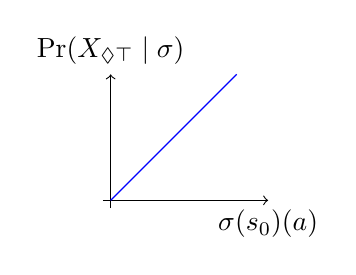
\begin{tikzpicture}[scale=2]
 \draw[->] (-0.05, 0) -- (1, 0) node[below]{$\sched(s_0)(a)$};
  	\draw[->] (0, -0.05) -- (0, 0.8) node[above] {$\Pr(X_{\lozenge\mathbf{\top}} \mid \sched)$};
  	%\draw[-,dashed] (0.4,0) -- (0.4,0.5184);
  	%\draw[-,dashed] (0.0,0.5184) -- (0.4,0.5184);
  \draw[ domain=0:0.8, smooth, variable=\x, blue] plot ({\x}, {\x});
\end{tikzpicture}
\caption{}
\end{subfigure}
\begin{subfigure}{0.38\columnwidth}
\centering
\begin{tikzpicture}[scale=2]	
 \draw[->] (-0.05, 0) -- (1, 0) node[below]{$\sched(s_0)(a)$};
  	\draw[->] (0, -0.05) -- (0, 0.8) node[above] {$H(\sched)$};
  	%\draw[-,dashed] (0.4,0) -- (0.4,0.5184);
  	%\draw[-,dashed] (0.0,0.5184) -- (0.4,0.5184);
 % \draw[ domain=0:1, smooth, variable=\x, blue] plot ({\x}, {15*(1-\x)*(1-\x)*(1-\x)*\x*\x});
\end{tikzpicture}
\caption{}
\end{subfigure}

\caption{Minimal ERCI problem.}
\end{figure}


Together, we obtain the following problem statement.
\begin{mdframed}[backgroundcolor=white!5]
\textbf{The ERCI Pareto Front Problem}:
Using the notation from the ERCI problem, find the set $\solutions \subseteq \mathbb{R}^2$.
\end{mdframed}
We are going to iteratively construct the  Pareto optimal points in $\solutions$. This yields a semi-decision procedure.
Clearly, finding $\solutions$ solves the ERCI problem, as we only need to decide whether $\langle \scthreshold, \randomness \rangle \in \solutions$.



With these facts, we are now well-equiped to develop the algorithms in Sec.~\ref{sec:mdp} for MDPs and Sec.~\ref{sec:sgs} for SGs.

Before we continue, we want to establish that Control improvisation problem is a conservative extension of deterministic case as investigated in~\cite{}.
\begin{mdframed}
\textbf{The Deterministic (Reactive) Control Improvisation (DCI) Problem~\cite{}}:
Given a \emph{deterministic} SG $\sg$, finite path sets $X_\psi$ and $X_\varphi$, and a threshold $p \in (0,1)$,  find a $\pOne$-policy $\pOneSched \in \POneScheds$  such that for every $\pTwo$-policy $\pTwoSched \in \PTwoScheds$ 
\begin{compactenum}
\item (\emph{hard constraint}) $\Pr(X_\psi \mid \sched) \geq 1$
	\item (\emph{soft constraint)} $\Pr(X_\varphi \mid \sched) \geq \scthreshold$
	\item (\emph{randomness constraint}) $\Pr(\path) \leq \delta \text{ for all } \path \in \Paths[h]{\sg[\sched]}$.
\end{compactenum}
\end{mdframed}

\begin{theorem}
	For deterministic SGs, the ERCI and DCI problem coincide.
\end{theorem}
We defer a discussion and a precise statement to Lemma~\ref{}.








\section{Maximum Entropy Traces and Policy Improvisation}
In this section, we discuss the nature of the randomness as imposed by the CI problem, and relate this to improvising policies, i.e., to randomly sampling policies that satisfy the hard and soft constraint.

\begin{mdframed}

\begin{compactenum}
	\item $\Pr^\sg_{\langle \sched_1,\sched_2 \rangle}(\eventually{h} T) \geq 1$
	\item $\Pr^\sg_{\langle \sched_1,\sched_2 \rangle}(\eventually{h} G) \geq \lambda$ 
\end{compactenum}
\end{mdframed}
\sj{Define randomly selected policy}




\section{Solving the Control Improvisation Problem for MDPs}
We present an algorithm for the control improvisation problem for MDPs. The key insight is to reuse ideas from policy inference from specifications~\cite{}. In the next section, we extend this idea to SGs.

\section{Solving the Control Improvisation Problem for SGs}

\section{Empirical Evaluation}

\end{document}
